\documentclass[12pt,a4paper,oneside]{article}

\usepackage{hyperref}
\usepackage{booktabs}
\usepackage{multirow}
\usepackage{multicol}
\usepackage{tabularx}
\usepackage[utf8]{inputenc}
\usepackage{graphicx}
\usepackage{caption}
\usepackage{subcaption}
\usepackage[margin=2.5cm]{geometry}
\usepackage[section]{placeins}
\graphicspath{{../figures/}}

\title{Predicting the Severity of a Traffic Collision}
\author{Jonathan Ström}
\date{October 11 \\ 2020}

\begin{document}

\maketitle

\section{Introduction}


\subsection{Background}

Traffic collisions can cause significant traffic delays and thus it is desirable to try to avoid these best one can. 
The purpose of this model is the predict the severity of a potential road accident, allowing the traveller to plan their trips . 
Collision severity will be predicted based on the road and light conditions at a given point in time. 

\subsection{Stakeholders}

This type of model is useful for anyone seeking to plan a trip and wish to avoid being stuck in traffic due to accidents. 
Perhaps it is especially useful for those who value avoiding wasting their time in traffic, and have the ability to plan their travelling. 
E.g., delivery drivers may not benefit as much for this model as, for instance, people travelling for leisure/vacation, as the former are often on a schedule outside of their control and may therefore be forced to travel irrespective of what the model suggests. 
However, the model can be used to plan deliveries (and the like) more carefully, and reduction of leisurely drivers during more accident prone times will still benefit those with less choice.

\section{Data}

\subsection{Source}

The data used in this work is from the Seattle Department of Transportation (SDOT). It contains information about all of the traffic collisions in Seattle from 2004 until present day (2020). The data was provided by the Seattle Police Department (SPD) and recorded by Traffic Records. The data is recorded in 
\href{https://github.com/jstr0em/coursera-capstone/blob/master/Data-Collisions.csv}{Data-Collisions.csv} with metadata in \href{https://github.com/jstr0em/coursera-capstone/blob/master/Metadata.pdf}{Metadata.pdf}.

\subsection{Target Variable}

The dataset contains a variable called SEVERITYCODE, which denotes how severe a collision was. 
This is our target variable, i.e. the value which we wish to predict. 
The meaning of each value of SEVERITYCODE can be seen in Table \ref{tbl:severitycode}.

\begin{table}[htbp!]
    \centering
    \caption{Overview of the target variable SEVERITYCODE.}
    \label{tbl:target_variable}
    \begin{subtable}[h]{\textwidth}
        \centering
        \caption{SEVERITYCODE and its corresponding meaning for traffic collision outcomes.}
        \label{tbl:severitycode}
        \begin{tabular}{l l}
            \toprule
            SEVERITYCODE & Meaning \\
            \midrule
            3 & Fatality \\
            2b & Serious injury \\
            2 & Injury \\
            1 & Property damage \\
            0 & Unknown \\
            \bottomrule
        \end{tabular}
    \end{subtable}

    \begin{subtable}[h]{\textwidth}
        \centering
        \caption{SEVERITYCODE and its number unique values.}
        \label{tbl:severitycode_count}
        \begin{tabular}{l l}
            \toprule
            SEVERITYCODE & Count \\
            \midrule
            1 & 136485 \\
            2 & 58188 \\
            \bottomrule
        \end{tabular}
    \end{subtable}

\end{table}

The number of unique SEVERITYCODE values can be seen in Table \ref{tbl:severitycode_count}. 
Here it is apparent that there actually only are two out of five SEVERITYCODE values present in the dataset - 1 and 2, or property damages and injuries respectively. 
We also note that there are far more cases of property damage than injuries; our dataset is unbalanced which may introduce a bias towards property damage, which will be addressed later. 


\subsection{Feature Selection}

The dataset contains 37 features and we need to select which ones to use to train and validate our model. 
Selection will occur through exclusion, and which features have been excluded and why is shown in Table \ref{tbl:feature_exclusion}.

\begin{table}[htbp!]
    \centering
    \caption{The excluded features with the reason for exclusion.}
    \label{tbl:feature_exclusion}
    \begin{tabularx}{\textwidth}{l X X}
        \toprule
        Feature & Meaning & Reason for exclusion \\
        \midrule\midrule
        OBJECTID & & \multirow{10}{=}{ID numbers} \\
        INCKEY & & \\
        COLDETKEY & & \\
        REPORTNO & & \\
        STATUS & & \\
        INTKEY & & \\
        EXCEPTRSNCODE & & \\
        EXCEPTRSNDESC & & \\
        SEVERITYDESC & & \\
        SDOTCOLNUM & & \\
        \midrule
        INCDATE & Incident date & \multirow{2}{=}{Dates/times} \\
        INCDTTM & Incident time& \\
        \midrule
        SEVERITYCODE.1 &  & Duplicate \\
        \midrule
        PEDCOUNT & Number of pedestrians involved & \multirow{18}{=}{Not useful for the predictive purposes outlined in this model. But may be useful for policymakers and automobile manufacturers.} \\
        PEDCYLCOUNT & Number of pedestrians and cyclists involved &  \\
        PERSONCOUNT & Number of people involved &  \\
        VEHCOUNT & Number of vehicles involved &  \\
        SPEEDING & Speeding &  \\
        UNDERINFL & Under the influence &  \\
        INATTENTIONIND & Inattentive driver &  \\
        PEDROWNOTGRNT & Not giving pedestrian right of way & \\
        ST\_COLCODE & \multirow{2}{=}{Car travelling direction prior to collision} & \\
        ST\_COLDESC & \\
        SDOT\_COLCODE & \multirow{2}{=}{Details of specific collision} & \\ 
        SDOT\_COLDESC & \\
        SEGLANEKEY & Lane segment collision occurred & \\
        CROSSWALKKEY & Collision  & \\
        HITPARKEDCAR & If a parked car was hit & \\
        COLLISIONTYPE & What the driver was doing while the accident occurred & \\
        JUNCTIONTYPE & Which junction type an accident occurred in & \\
        ADDRTYPE & Similar to JUNCTIONTYPE & \\
        \midrule
        X \& Y & Collision coordinates & \multirow{2}{=}{Not relevant for this model scope} \\
        LOCATION & Detailed location description &  \\
        \bottomrule
    \end{tabularx}
\end{table}

After the features in Table \ref{tbl:feature_exclusion} has been removed, the features in Table \ref{tbl:feature_selection} remain and will be used for training and testing the model. 

\begin{table}[htbp!]
    \centering
    \caption{Selected features for training and testing the model.}
    \label{tbl:feature_selection}
    \begin{tabular}{l l}
        \toprule
        Feature & Meaning \\
        \midrule
        LIGHTCOND & Lighting conditions at the time of the collision \\
        ROADCOND & Road conditions at the time of collision \\
        WEATHER & Weather at the time of collision \\
        \bottomrule
    \end{tabular}
\end{table}

\section{Methodology}

\subsection{Exploratory Data Analysis}

All of the features and target variable of the dataset are categorical, thus a count of how each feature value grouped by each unique target variable value is performed.
The result of these can be seen in Table \ref{tbl:feature_count}, which show the aforementioned analysis for WEATHER, LIGHTCOND, and ROADCOND; Figure \ref{fig:feature_count} shows the same as the tables, but as a figure.

By observation, we notice that the vast majority of collisions (regardless of severity) seem to occur during what would be considered good conditions - daylight, clear weather, and dry roads. 
This is likely due to the fact that the majority of travels occur during these conditions (especially daylight), so this is to be expected. 
We also note again that during these times, collisions resulting in property damage are more common than injuries. 
This (again) highlights the unbalanced nature of the dataset, and how there might be a challenge to use the more rare features for prediction - which is why we will use an under-sampling scheme in the preprocessing state.

There also are a few cases labeled as Unknown or Other in all of the features, these will be difficult to use as an user input for prediction. 
Thus, the corresponding cases will be removed from the training and testing sets. 

\begin{table}[htbp!]
    \centering
    \caption{Count of each feature value grouped by the target variable SEVERITYCODE.}
    \label{tbl:feature_count}
    % WEATER
    \begin{subtable}[h]{\textwidth}
        \centering
        \caption{WEATHER feature.}
        \label{tbl:weather}
        \begin{tabular}{l c c}
            \toprule
            \multirow{2}{*}{WEATHER} & SEVERITYCODE \\
            \cmidrule{2-3}
            & 1 & 2 \\
            \midrule
            Blowing Sand/Dirt & 40 & 15 \\
            Clear & 75200 & 35808 \\
            Fog/Smog/Smoke & 382 & 187 \\
            Other & 708 & 116 \\
            Overcast & 1894 & 8739 \\
            Partly Cloudy & 2 & 3 \\
            Raining & 21949 & 11168 \\
            Severe Crosswind & 18 & 7 \\
            Sleet/Hail/Freezing Rain & 85 & 28 \\
            Snowing & 732 & 169 \\
            Unknown & 14227 & 812 \\
            \bottomrule
        \end{tabular}
    \end{subtable}
    % LIGHTCOND
    \begin{subtable}[h]{\textwidth}
        \centering
        \caption{LIGHTCOND feature.}
        \label{tbl:lightcond}
        \begin{tabular}{l c c}
            \toprule
            \multirow{2}{*}{LIGHTCOND} & SEVERITYCODE \\
            \cmidrule{2-3}
            & 1 & 2 \\
            \midrule
            Dark - No Street Lights & 1201 & 334 \\
            Dark - Street Lights Off & 876 & 316 \\
            Dark - Street Lights On & 33989 & 14451 \\
            Dark - Unknown Lighting & 7 & 4 \\
            Dawn & 1678 & 824 \\
            Daylight & 77549 & 38528 \\
            Dusk & 3951 & 1938 \\
            Other & 183 & 52 \\
            Unknown & 12851 & 605 \\
            \bottomrule
        \end{tabular}
    \end{subtable}
    % ROADCOND
    \begin{subtable}[h]{\textwidth}
        \centering
        \caption{ROADCOND feature.}
        \label{tbl:roadcond}
        \begin{tabular}{l c c}
            \toprule
            \multirow{2}{*}{ROADCOND} & SEVERITYCODE \\
            \cmidrule{2-3}
            & 1 & 2 \\
            \midrule
            Dry & 84296 & 40004 \\
            Ice & 933 & 273 \\
            Oil & 40 & 24 \\
            Other & 88 & 43 \\
            Sand/Mud/Dirt & 51 & 23 \\
            Snow/Slush & 833 & 166 \\
            Standing Water & 85 & 30 \\
            Unknown & 14284 & 747 \\
            Wet & 31675 & 15742 \\
            \bottomrule
        \end{tabular}
    \end{subtable}
\end{table}


\begin{figure}[htbp!]
    \centering
    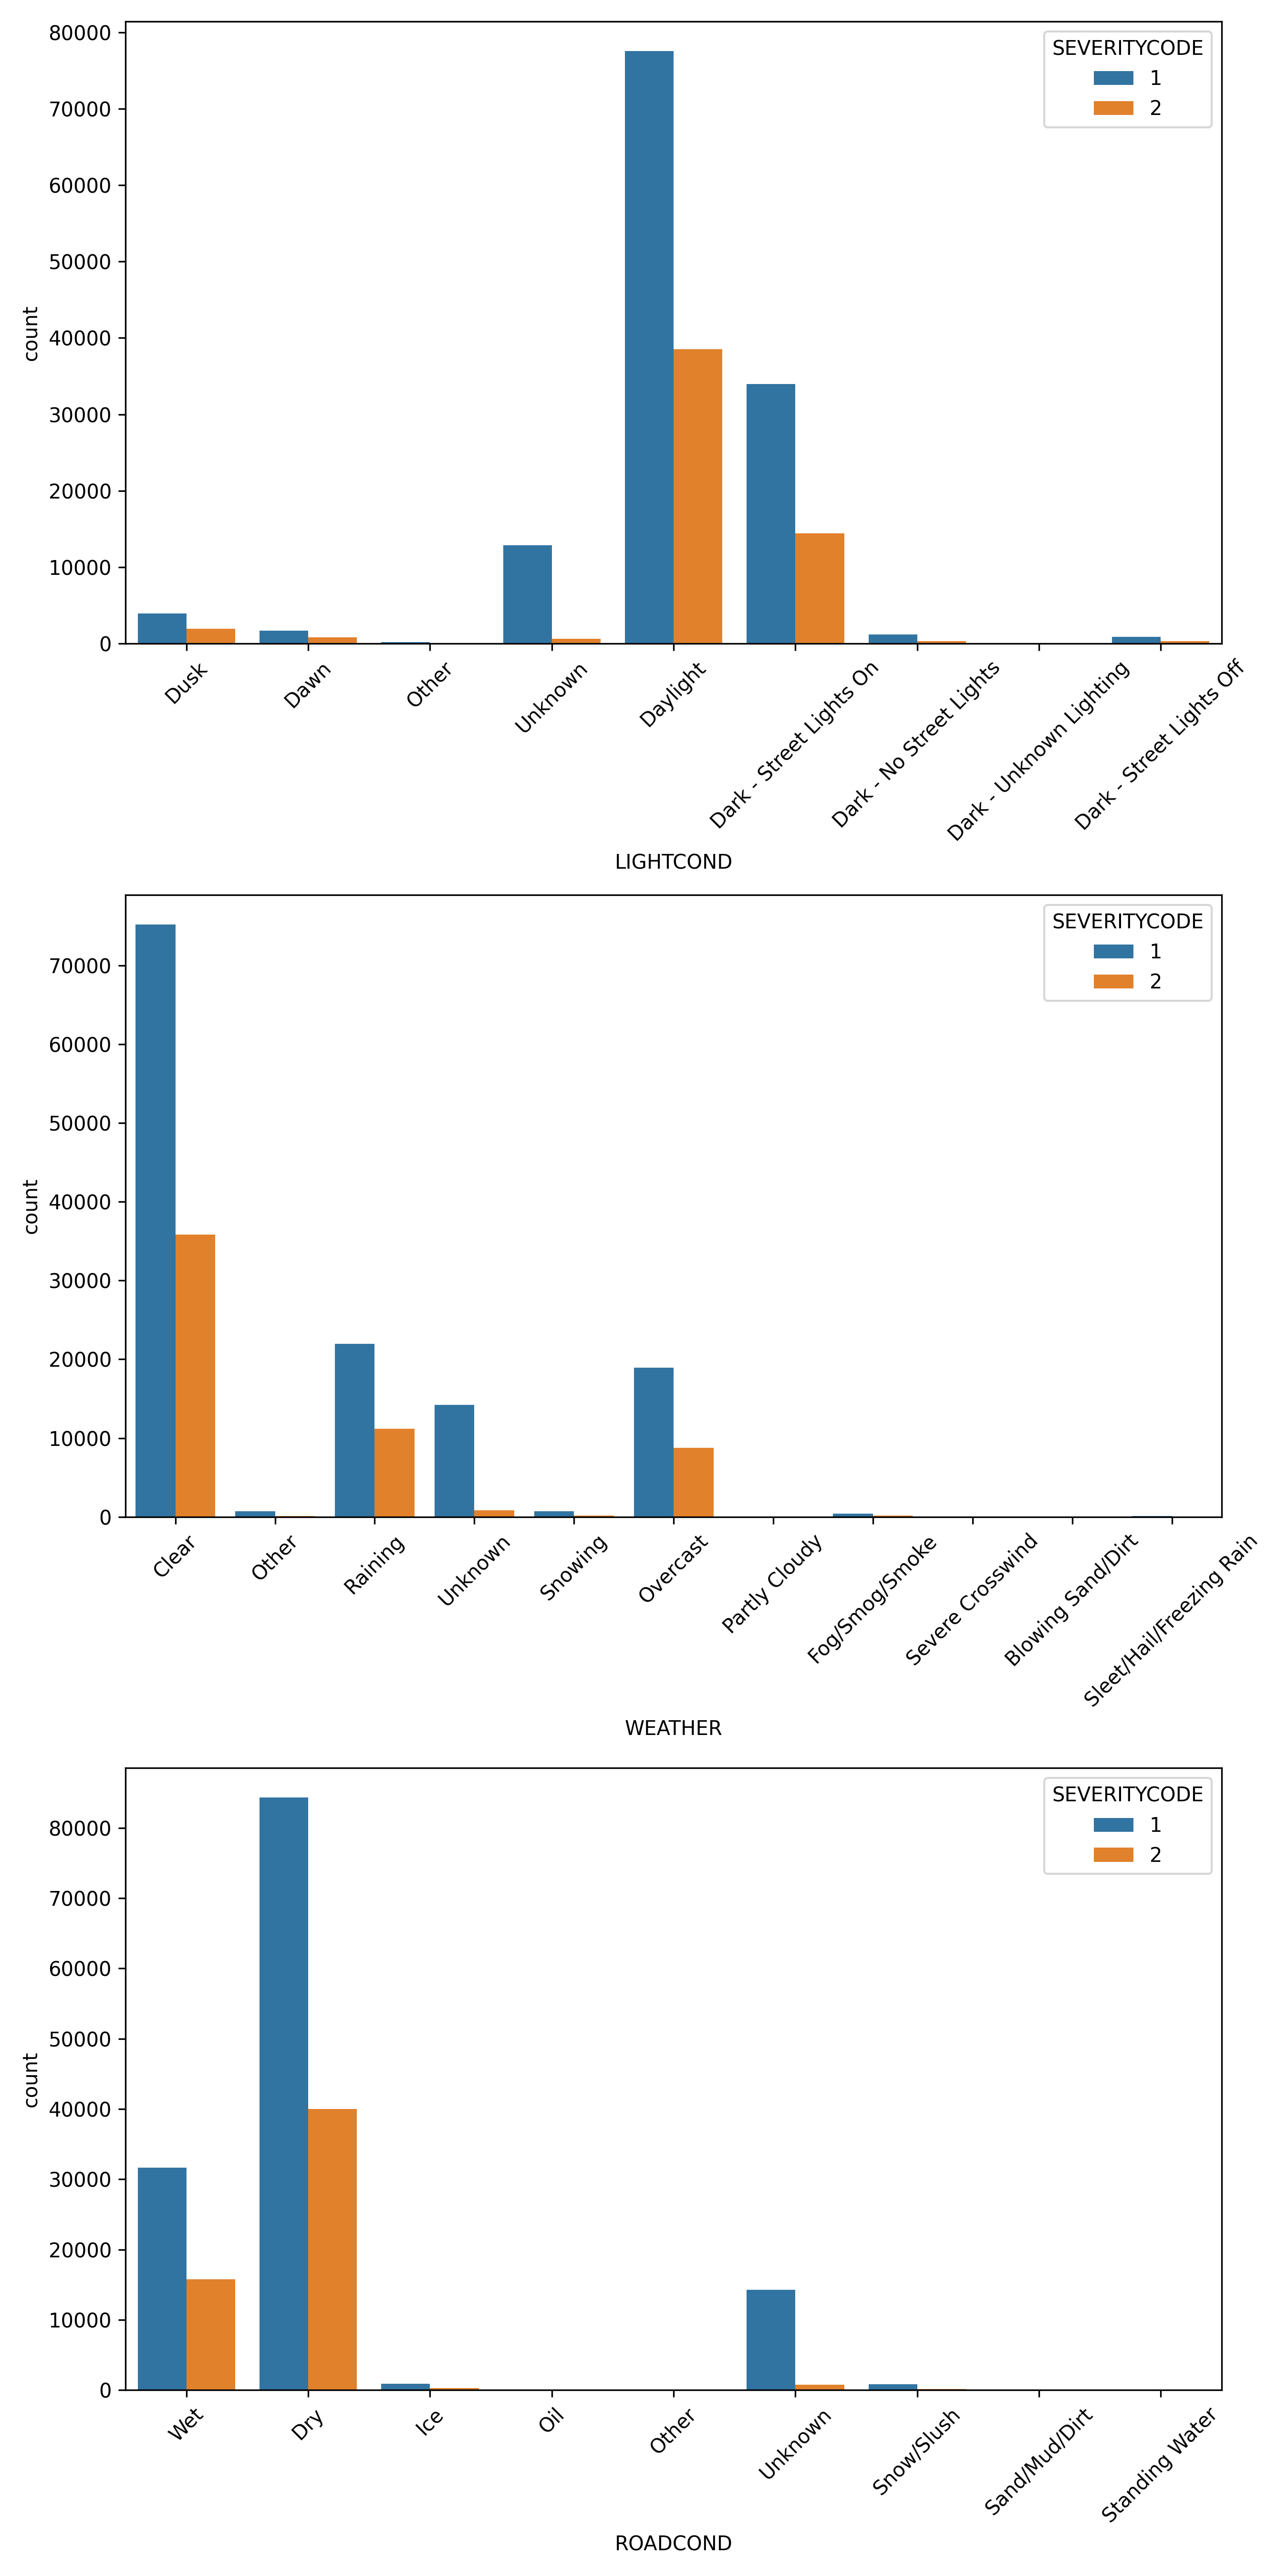
\includegraphics[height=0.95\textheight]{feature_count.png}
    \caption{Count of each feature value grouped by the target variable SEVERITYCODE.}
    \label{fig:feature_count}
\end{figure}

\subsection{Preprocessing}

The data preprocessing consists of steps outlined in Table \ref{tbl:preprocessing}.

\begin{table}[htbp!]
    \centering
    \caption{Data preprocessing steps taken before use for training and testing the model.}
    \label{tbl:preprocessing}
    \begin{tabularx}{\textwidth}{l X X}
        \toprule
        Step & Action & Reason \\ 
        \midrule
        1. & Remove cases that has a feature value of Unknown or Other. & No predictive utility. \\ 
        2. & One-hot encode features. & Categorical variables require conversion to some numeric value. We use one-hot encoding to avoid the model to rank any of the feature values according to some numeric rank. \\
        3. & Split dataset into a training and testing set. & We reserve 20\% of the data for testing. \\
        4. & Create a copy of the training set and resample it using an under-sampling scheme. & The dataset is unbalanced. To address this, we under-sample a copy of the training set to ensure that there are equal number of SEVERITYCODE entries; the most common case is under-sampled. The resulting dataset has 44,495 entries per SEVERITYCODE. \\
        \bottomrule
    \end{tabularx}
\end{table}


\subsection{Modeling}

All of the features and the target variable are all categorical, thus a supervised classification model is an appropriate choice.
There are many choices available, but in this work we will use Logistic Regression and Linear SVC as models. 
Two are chosen to compare their performances. 
These two are chosen as they are relatively fast choices (in terms of computation time).
For each of these models, we will train them on the unbalanced and balanced training sets to see which is more appropriate for fulfilling our purpose.
We will also use the default SKLearn modeling parameters.


\section{Results and Discussion}

Models analysis is done by producing a confusion matrix for each of the two models (linear SCV and logistic regression) trained on the two datasets (balanced and unbalanced).
The accuracy, recall, and F1-score of each model is also calculated.
All of this information is shown in Figure \ref{fig:confusion_matrix}.

Looking at the two models with their two respectively unbalanced and balanced datasets, we see that there is quite a lot going on. 
One thing that immediately stands out is that for the given unbalanced/balanced dataset, the models perform more or less equally in terms of their predictions and associated scores. 
However, we see that the models perform drastically differently depending on if the unbalanced or balanced dataset was used for training. 

When the unbalanced dataset was used, we see that the models never predict that a SEVERITYCODE = 2 collision occurs, i.e. all collisions will only result in property damage (and thus less severe traffic jams). 
Despite this inability to predict more serious collisions, the accuracy scores are quite good. 
This is a problem for our applications however, as we will always miss any serious collisions and thus defeat the purpose of this model - to avoid being stuck in traffic. 

In this case, it is better to be much more conservative in our predictions, i.e. it is better to overpredict the probability of a SEVERITYCODE = 2 collision. 
This is of course assuming that a more serious collision will result in much longer traffic delays (which seems quite reasonable). 

With the balanced dataset used for training, we see that our overall scores decrease significantly, and in fact are not that good. 
However, like discussed, we do predict far more serious collisions, giving these models a more conservative estimation of the risk of a collision. 
This is preferable for our purposes; \textbf{despite the poorer accuracy metrics, the models trained using the balanced datasets are preferable.}

\begin{figure}[htpb!]
    \centering
    \caption{Confusion matrix of the two models trained on the balanced and unbalanced datasets respectively.}
    \label{fig:confusion_matrix}
    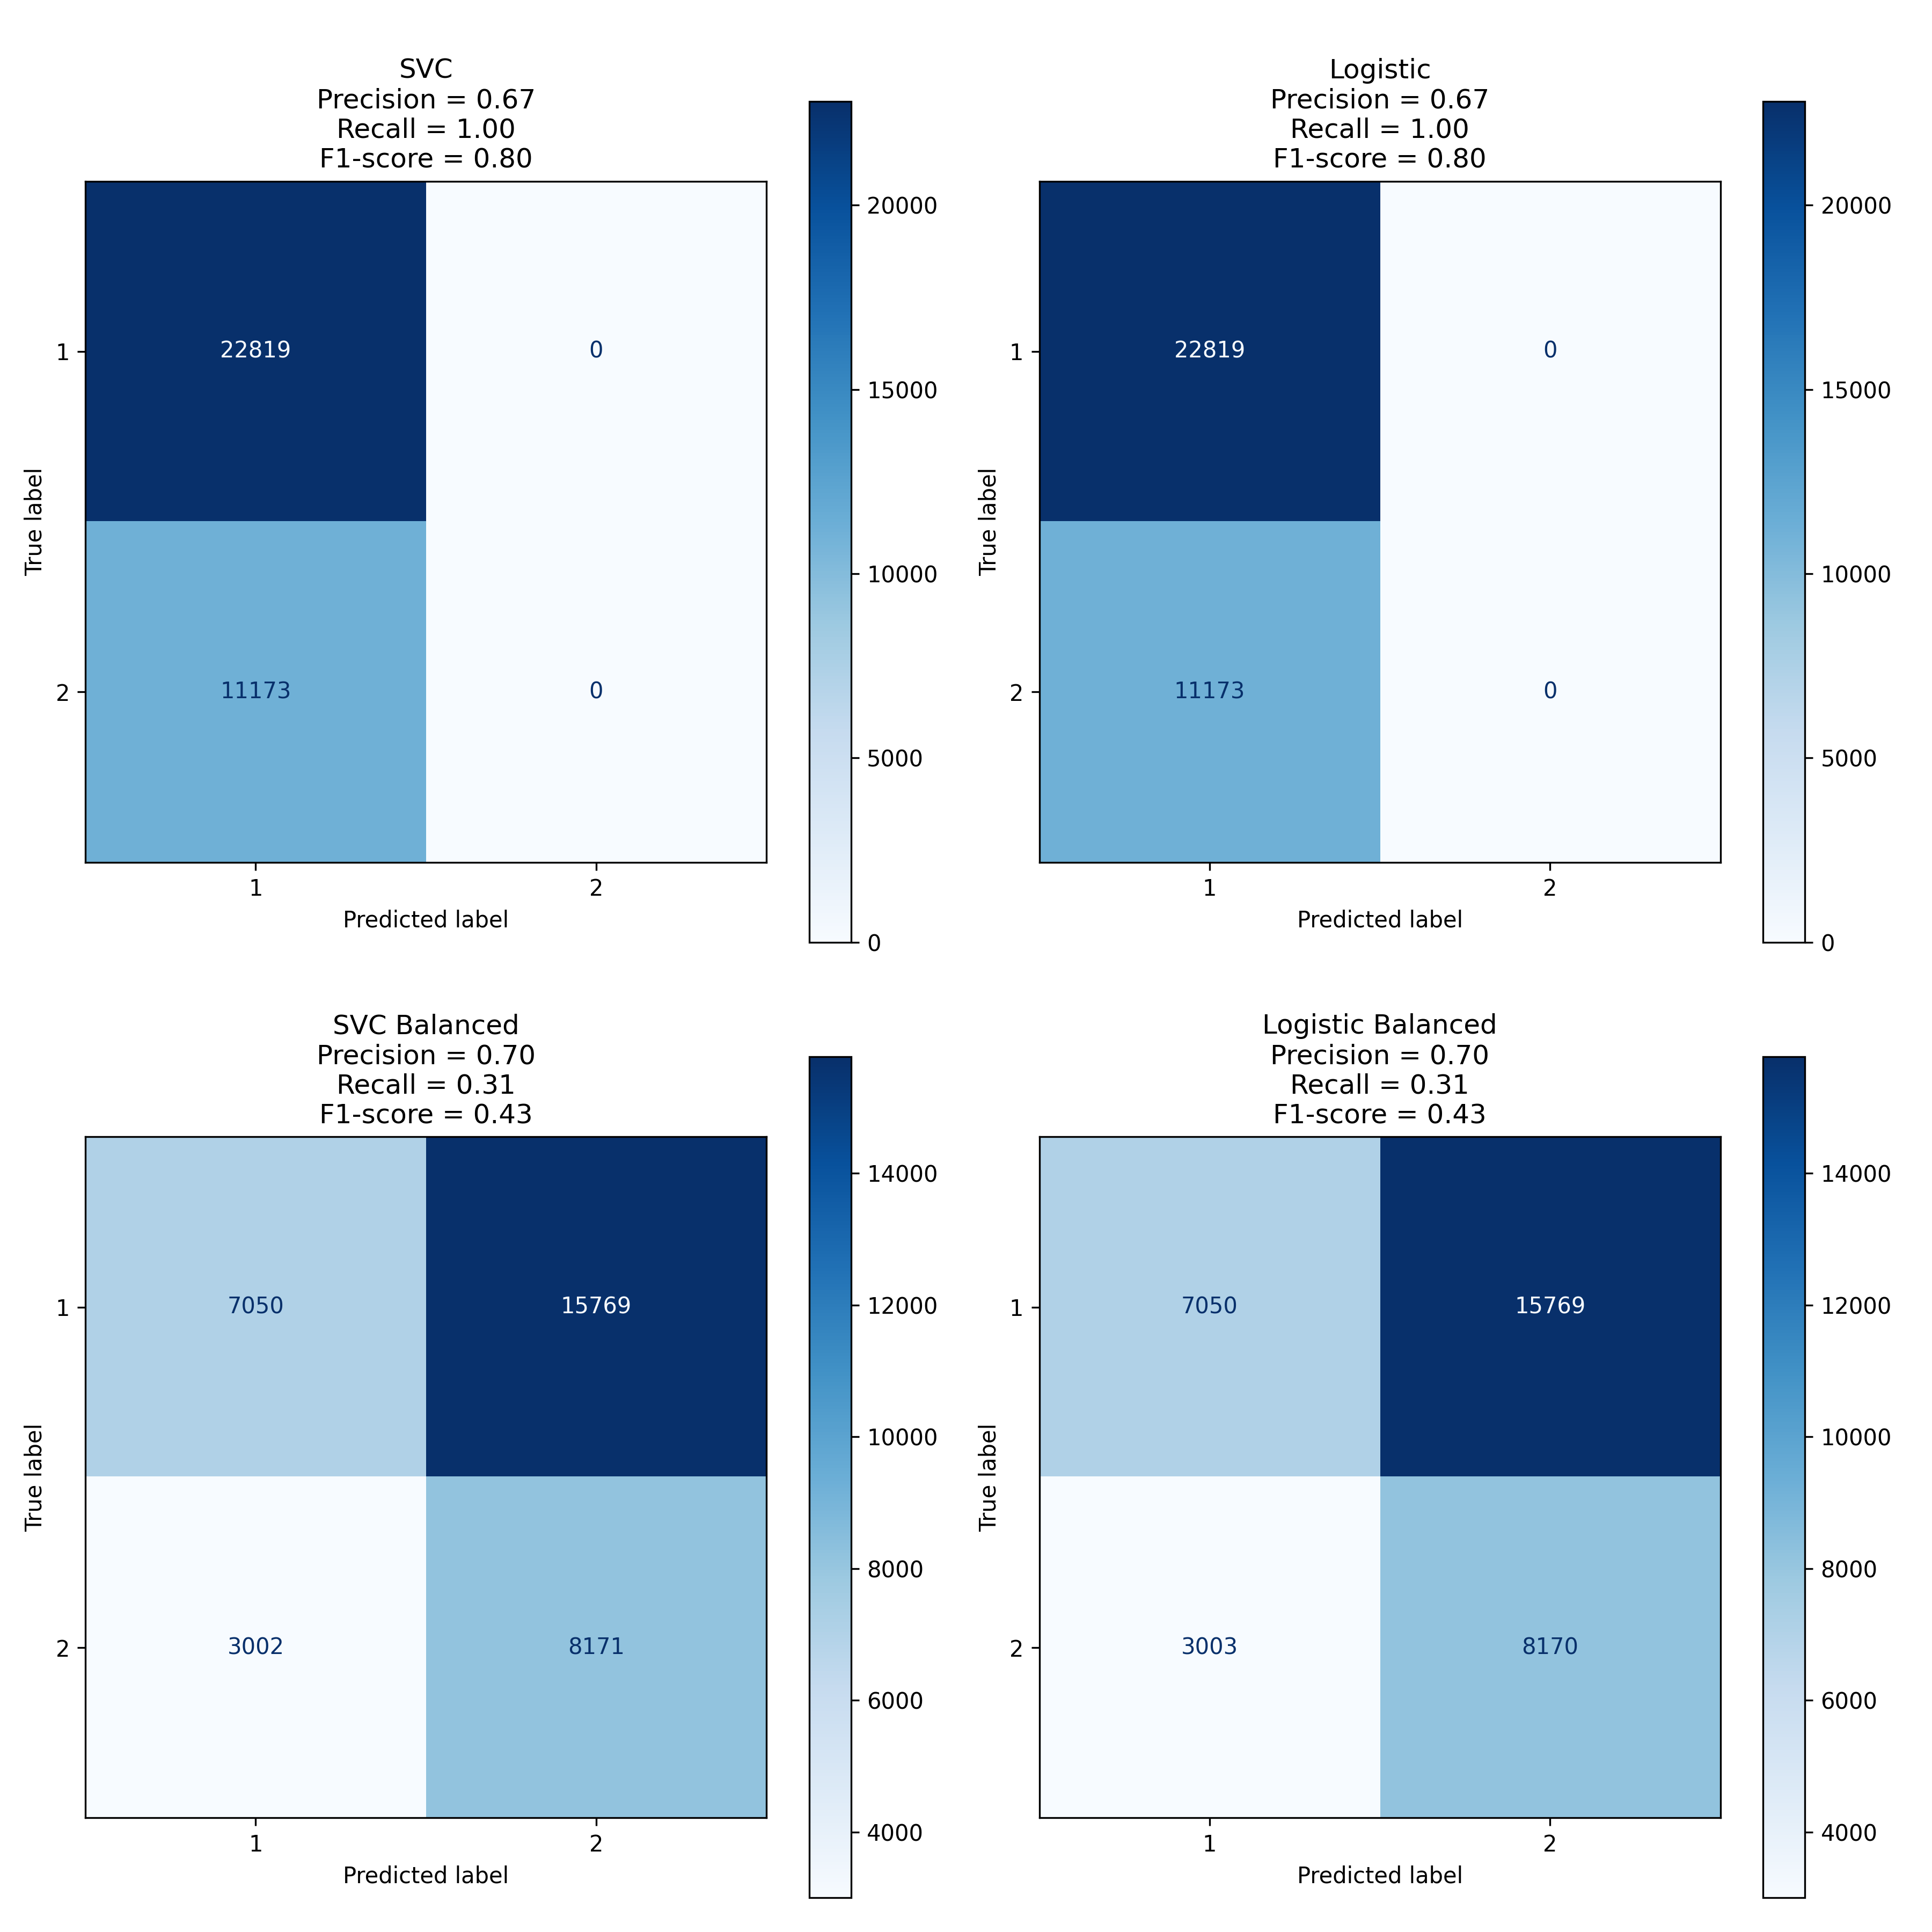
\includegraphics[width=\textwidth]{confusion_matrix.png}
\end{figure}

\subsection{Relative Feature Importance} 

From \ref{fig:feature_importance}, we can see which features with the largest importance for predictions of the two models. As we noted before, the two models trained on the balanced dataset performed almost identically in their predictions and their associated scores. Interestingly, these similarities do not extend to feature importance, and we can see that different features are deemed most important for predictions. Determining which one is more "right" is difficult to access without additional information, but the results are reasonably similar; more rare and extreme phenomena are typically more important - which makes intuitive sense. 

\begin{figure}[htpb!]
    \centering
    \caption{Relative importance of the features for the two given models. Here only the models trained on the balanced dataset are considered.}
    \label{fig:feature_importance}
    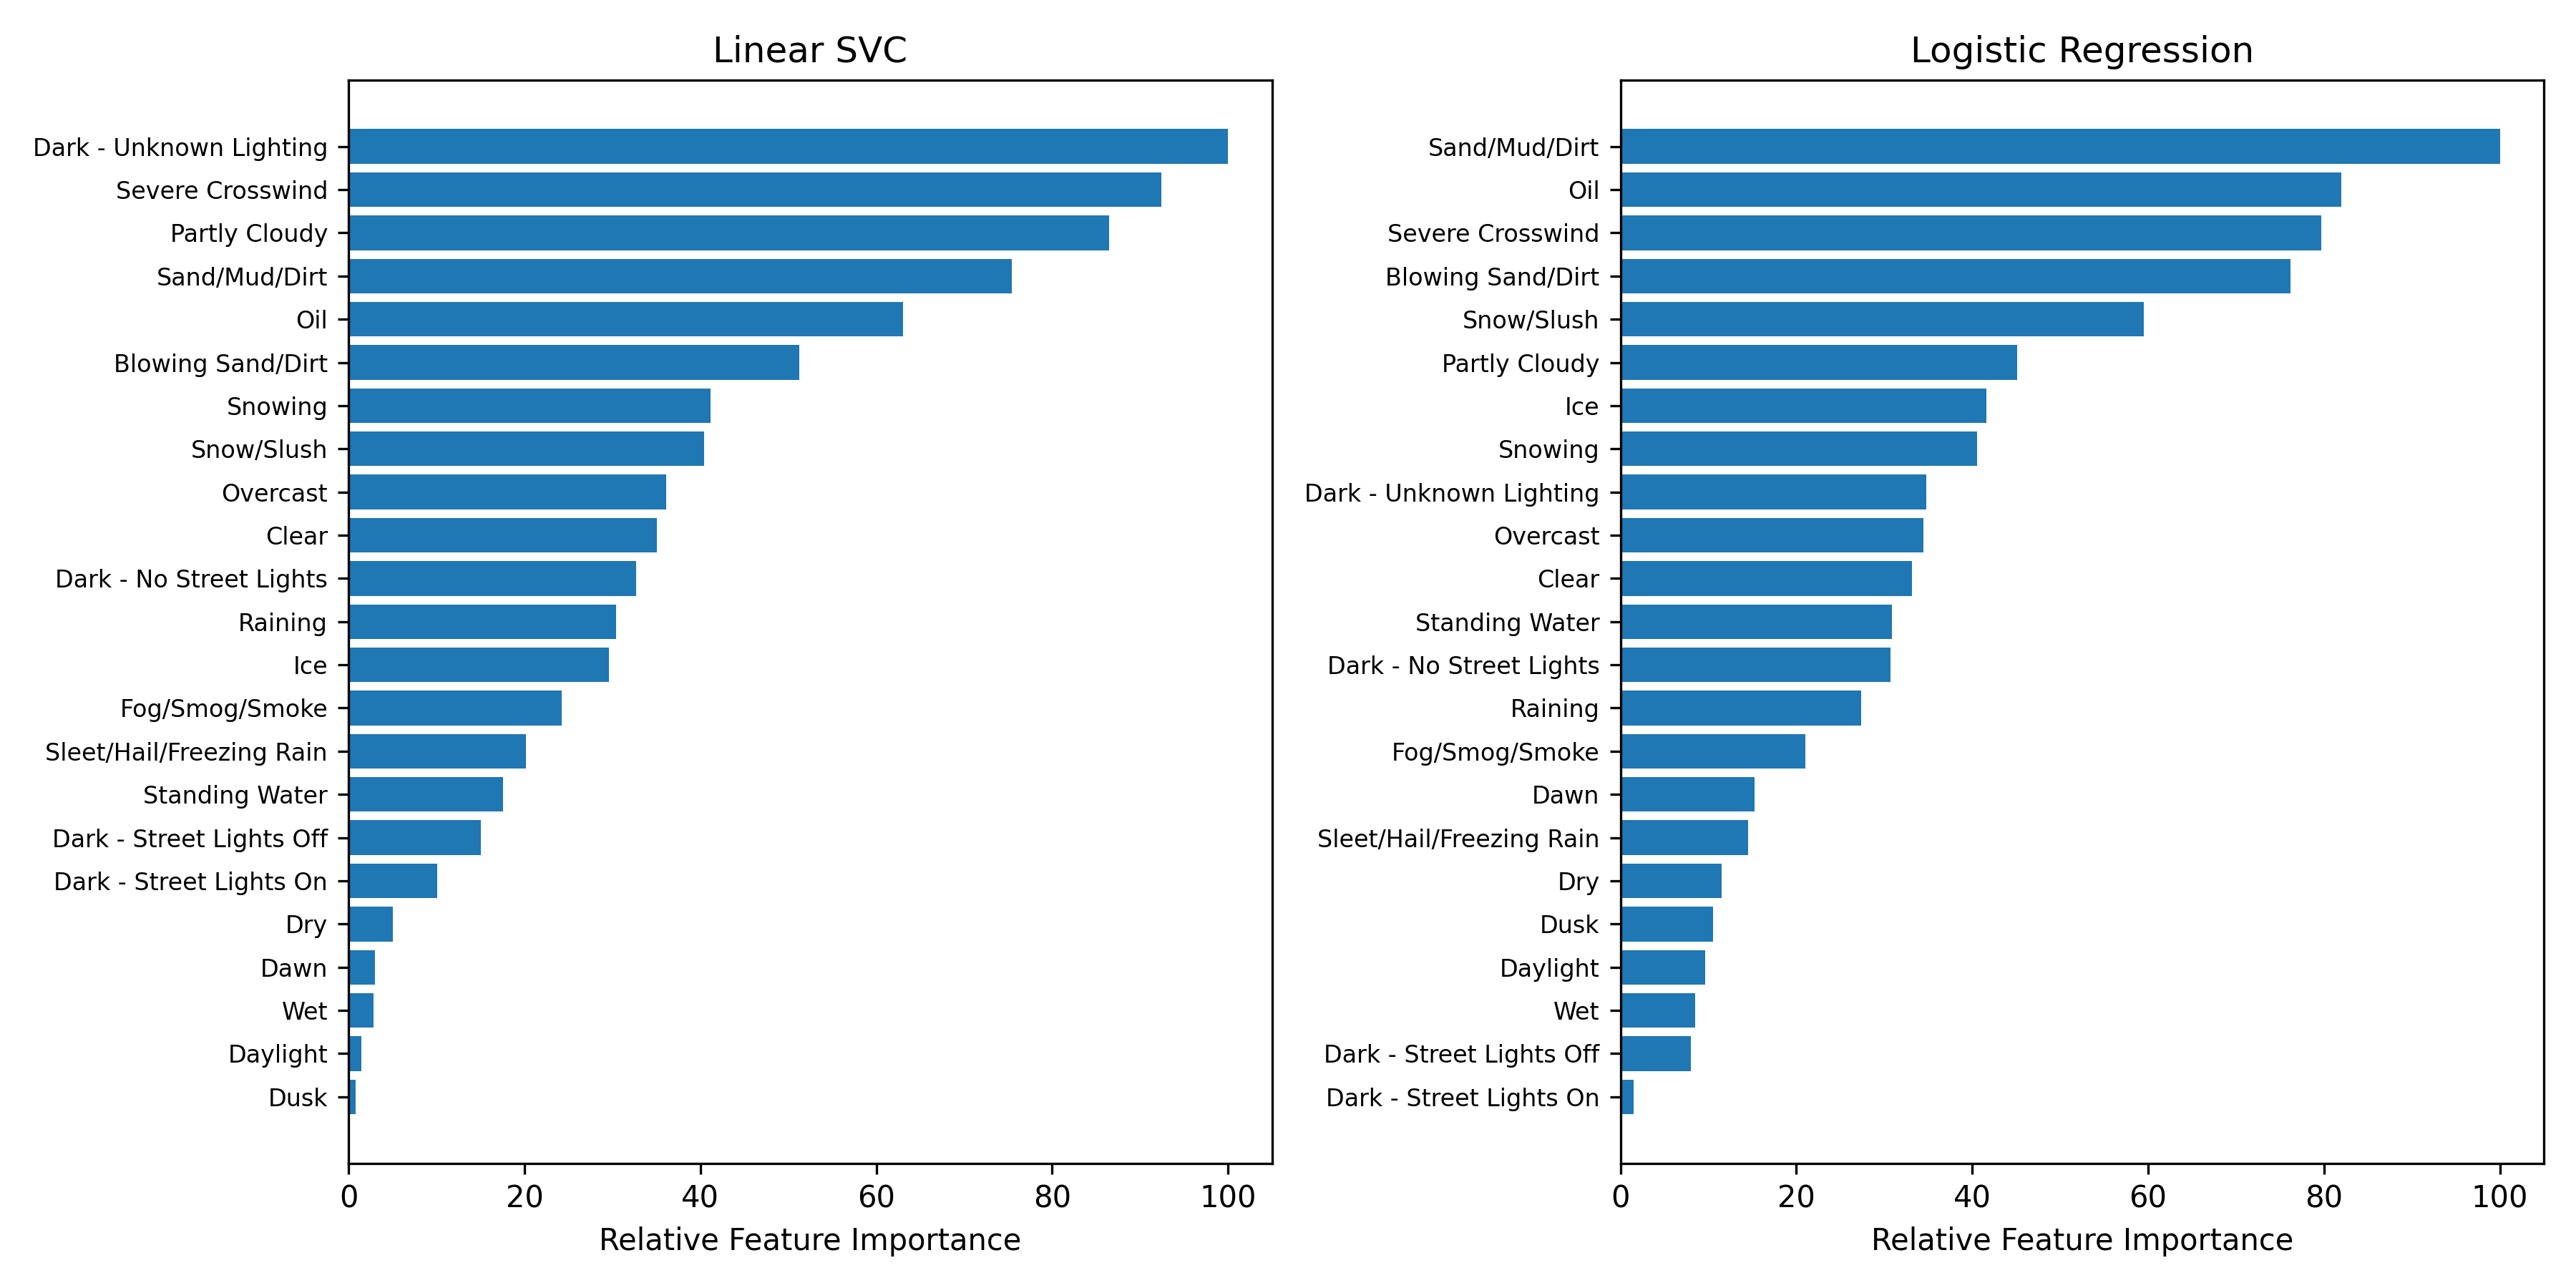
\includegraphics[width=\textwidth]{feature_importance.png}
\end{figure}

\subsection{Potential Limitations of Model}

While the data used to create the model is based on traffic accident data in Seattle, it is likely that the model is generalizable to situations outside of Seattle as well. 
However, this predictive ability likely decreases as the predicted area becomes more different from Seattle. 
For instance, Seattle is located in the Pacific Northwest of the United States, and the model will likely perform best for areas that has similar driving laws/cultures and climate as Seattle does. 
Thus, this model is most useful to stakeholders travelling through areas of this type. 
 
Another limitation is that there are only two type of collisions in the dataset - property damage and injuries. This is obviously a problem as it is impossible to predict other types of collision outcomes. 

\section{Conclusions}

In this study, we have designed a model that predicts the severity of a road collision based on the weather, road conditions, and lighting conditions. 
The purpose of this is to allow the user to plan their travels in such a way to reduce the chance of more severe accidents occurring, and thereby reducing their time in traffic caused by these accidents. 
Due to limitations in the dataset, it is only possible to predict one out of two classes of collisions, either ones resulting in only property damage (less severe accidents) or those resulting in injuries (more severe accidents). 
Two classification models were used in this work - linear SVC and logistic regression, and according to the measured metrics, both of these performed equally well for this application. 

The dataset was significantly unbalanced, and accidents resulting in property damage were much more common than those resulting in injuries. 
This necessitated the resampling of the dataset to contain equal number of types of collisions, otherwise a heavy bias for less severe accidents would be introduced, and thus eliminating the utility of this model. 
The resampling had the effect of instead creating a bias towards more significant accidents. 
This was deemed preferable, as it is better to be overly conservative in this application. 

The modeling also revealed which conditions are most important in our models. 
While the exact feature importance ranking within each model differed somewhat, both agreed that more extreme conditions are relatively more important, e.g. driving in the dark, during snow, or heavy wind. 
These results are not that surprising, but is an important "sanity check" to see if our model predictions make sense. 
\end{document}
